\chapter{Experiment description}
\label{chap:experiment}

\section{The task}
    The subjects were 8 adult naive male Wistar rats (12 - 16 weeks old, 380 - 400g). The animals were housed individually in a 12h light/dark cycle with the light turned on at 7am, and put under food deprivation to gradually reach and maintain 85\% of their free-feeding weight. Animals were handled according to the experimental protocol approved by the Committee of Ethics in Animal Usage from UFABC (CEUA-UFABC). All procedures were conducted during the light cycle.
    
    Animals were trained in an operant chamber developed in our laboratory, totally controlled by an Arduino uno, and made of acrylic plastic. The box has a \textit{nosepoke}, which is a hole equipped with an infrared emitter-sensor that detects when the animal pokes inside. In the same wall there is a drinker coupled to a lickometer, to which the animal has its access limited by a gate controlled by a stepper motor.
    
    \begin{figure}
        \centering
        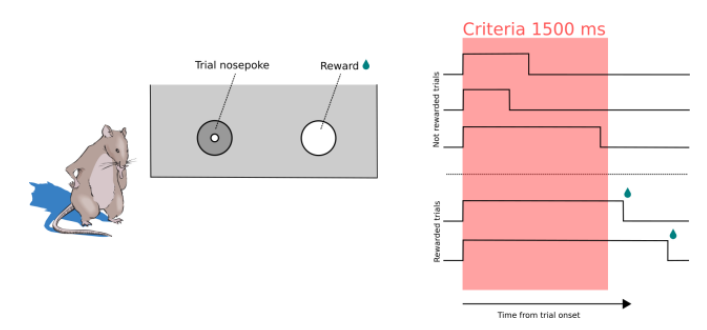
\includegraphics[width=\textwidth]{figures/tarefa_eli.png}
        \caption[Our DRRD task]{Our DRRD task. If the animal stays in the nosepoke for longer than the criteria, it can collect a reward. Taken with permission from \cite{Eliezyer2018}}
        \label{fig:task}
    \end{figure}

\section{Training}
    First, the animals were trained to nose poke the hole through a continuous schedule of reinforcement (CR), in which every nosepoke is rewarded independent of duration. To conclude this phase the animal had to nose poke the hole at least 100 times on a 60 minutes session. 
    After reaching this performance, on the next day, the animals were trained with a Differential Reinforcement Response Duration (DRRD) procedure: The trials were self initiated and self ended. In order to receive reward (four licks of a 50\% glucose solution), the animal had to poke the hole and hold for a time equal or longer than the defined criterion of 1500ms. If the animal didn't reach the time criteria there is no reward, and it is free to start a new trial at any time. All sessions were video recorded.

\section{Rationale}
    The central distinction of this DRRD task is the speed of behavior acquisition. It was developed by our group to enable recording of neurons through learning in a single session, and most of the specifics of this task were defined with this aim.
    
    The original DRRD task has a window of reinforcement with criteria for minimum and maximum time, thus if the animal holds nosepoking for too long it receives no reward. We removed this second criterion to speed up training \cite{}, and justify that the challenge the subjects engage with is still one of timing -- as opposed to impulse control and waiting for as long as possible. We argue that the incentive to get reward as soon as possible is an intrinsic one, and thus we need not enforce a penalty for long responses. In fact, behavioral results indicate this is the case: animals' responses peak around the criterion, and very long responses are uncommon.